\normaltrue
\correctionfalse

%\UPSTIidClasse{11} % 11 sup, 12 spé
%\newcommand{\UPSTIidClasse}{12}

\exer{Fauteuil bateau $\star$ \label{A5:05:85}}
\setcounter{question}{0}\UPSTIcompetence[2]{A5-05}
\UPSTIcompetence[2]{A5-04}

\index{Compétence A5-05}
\index{Compétence A5-04}

\index{GPS}
\index{Spécification géométrique des produits}
\index{Roue motrice}

\ifcorrection
\else
\textbf{Pas de corrigé pour cet exercice.}
\fi

%\fi
\section*{Mise en situation}
\ifprof
\else
\fi

L'objet de l'étude est un << siège motorisé >> destiné à des navites de luxe. Cette motorisation permet de rendre le siège plus ergonomique. On s'intéresse en particulier ou basculement avant -- arrière du fauteuil.

\begin{center}
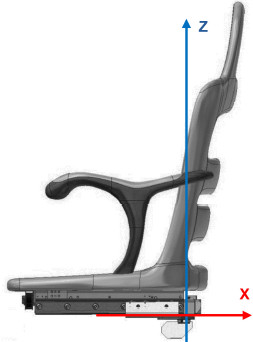
\includegraphics[height=3.5cm]{85_02}
\hspace{1cm}
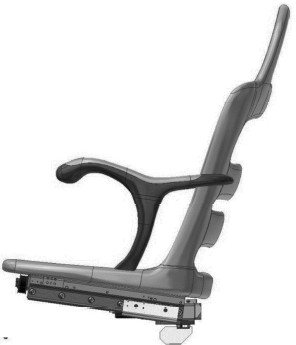
\includegraphics[height=3.5cm]{85_03}
\hspace{1cm}
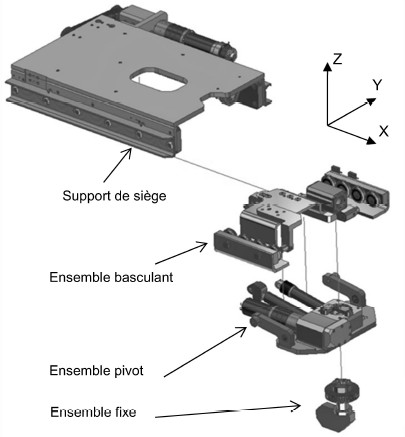
\includegraphics[height=3.5cm]{85_04}
\end{center}

L'ensemble étudié est constitué d'un ensemble fixe (lié au bateau), d'un ensemble pivot, basculant et du support de siège.

La chappe, objet des questions qui suivent, permet de faire la liaison entre l'ensemble pivot et l'ensemble basculant. 

\subsection*{Analyse des spécifications}
\question{Justifier pourquoi $A$, $B$ et $C$ sont utilisées comme surface de référence ?}

\question{Comment peut-on justifier fonctionnellement l'existence des spécifications suivantes 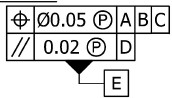
\includegraphics[width=.12\linewidth]{85_gps_00} ?}



\question{Analyser les spécifications suivantes
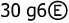
\includegraphics[width=.1\linewidth]{85_gps_01},
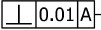
\includegraphics[width=.1\linewidth]{85_gps_02},
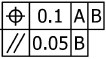
\includegraphics[width=.1\linewidth]{85_gps_03}. On note que $30 g6 = 30^{\begin{array}{c}-7 // -13\end{array}}$ (IT en $\mu$m.)}


\question{Quel serait l'effet d'un modificateur au maximum de matière sur l'exigence de localisation ? (exigence du maximum de matière porté sur la tolérance).}


\subsection*{Analyse des procédés de fabrication}

\question{Après avoir proposé un (ou plusieurs) moyens d'obtention du brut, préciser les différents étapes de fabrication de la chape.}

\question{Proposer une gamme de fabrication ainsi que les mises en position associées à chacun des phases.}



\begin{center}
{\rotatebox{270}{\includegraphics[height=\linewidth]{85_Dessin}}}
\rotatebox{0}{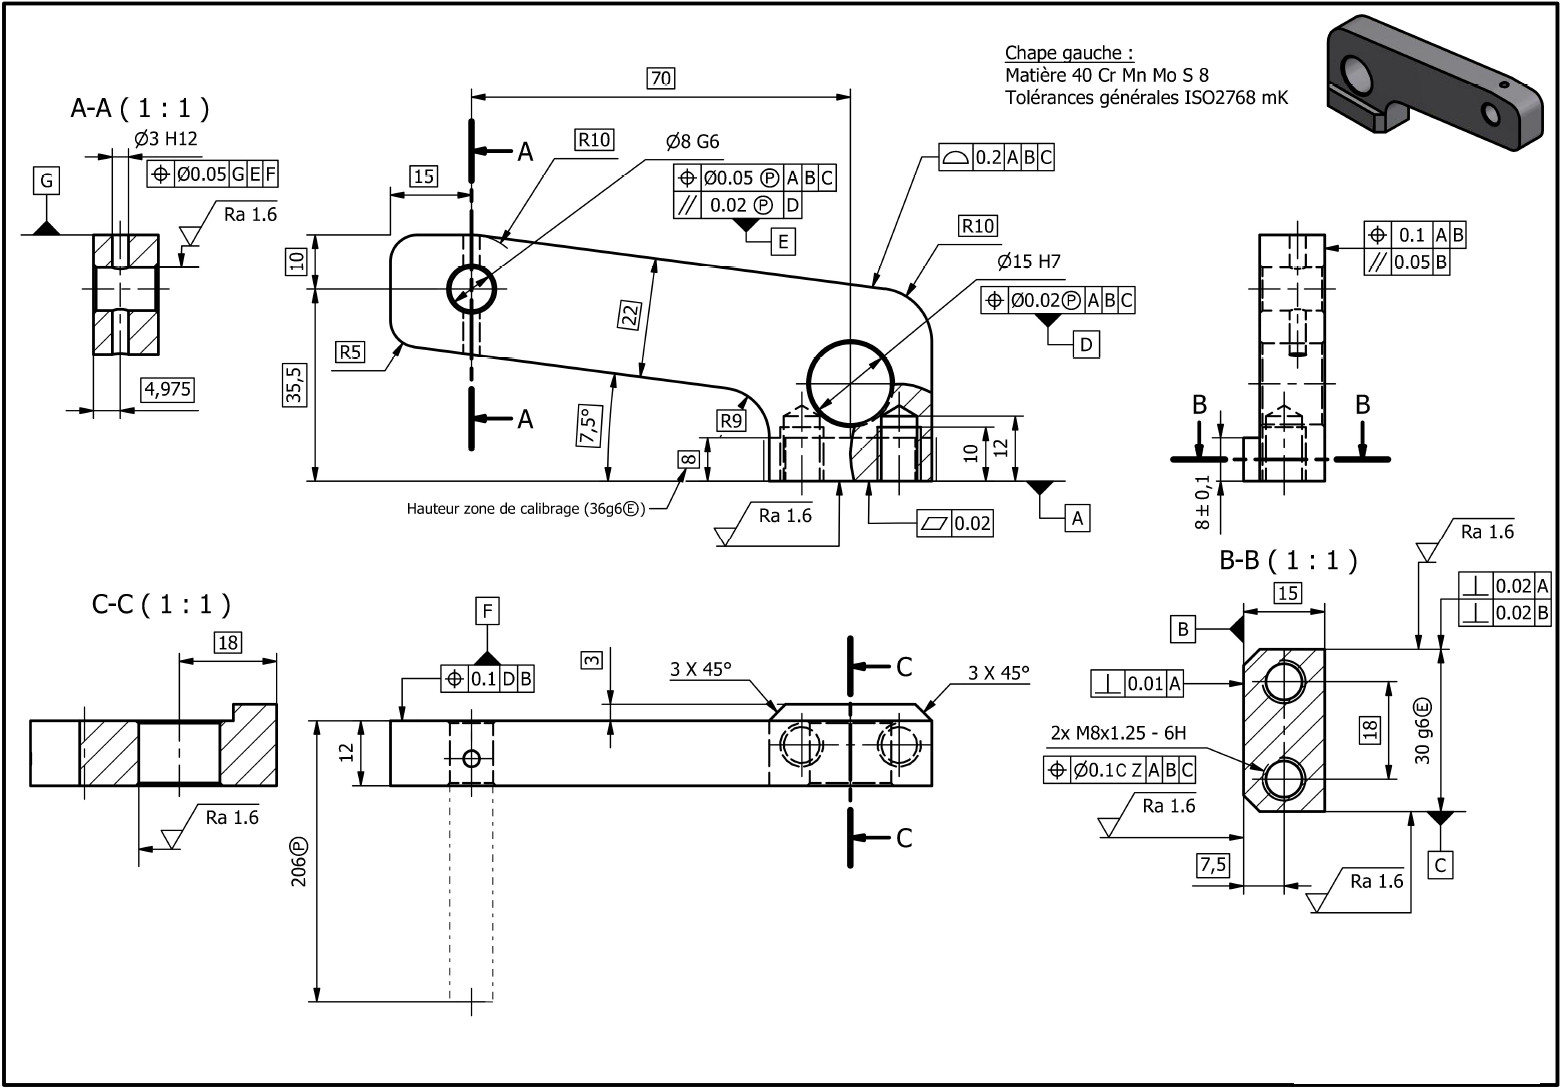
\includegraphics[width=\linewidth]{85_06}}
\end{center}



\ifprof
\else
\begin{flushright}
\footnotesize{Corrigé  voir \ref{A5:05:85}.}
\end{flushright}%
\fi 